\documentclass[border=10pt]{standalone}

\usepackage{tikz}
\usepackage{tikzsymbols}
\usetikzlibrary{calc,patterns,shapes.geometric}

\def\centerarc[#1](#2)(#3:#4:#5){\draw[#1] ($(#2)+({#5*cos(#3)},{#5*sin(#3)})$) arc (#3:#4:#5);}

\begin{document}
	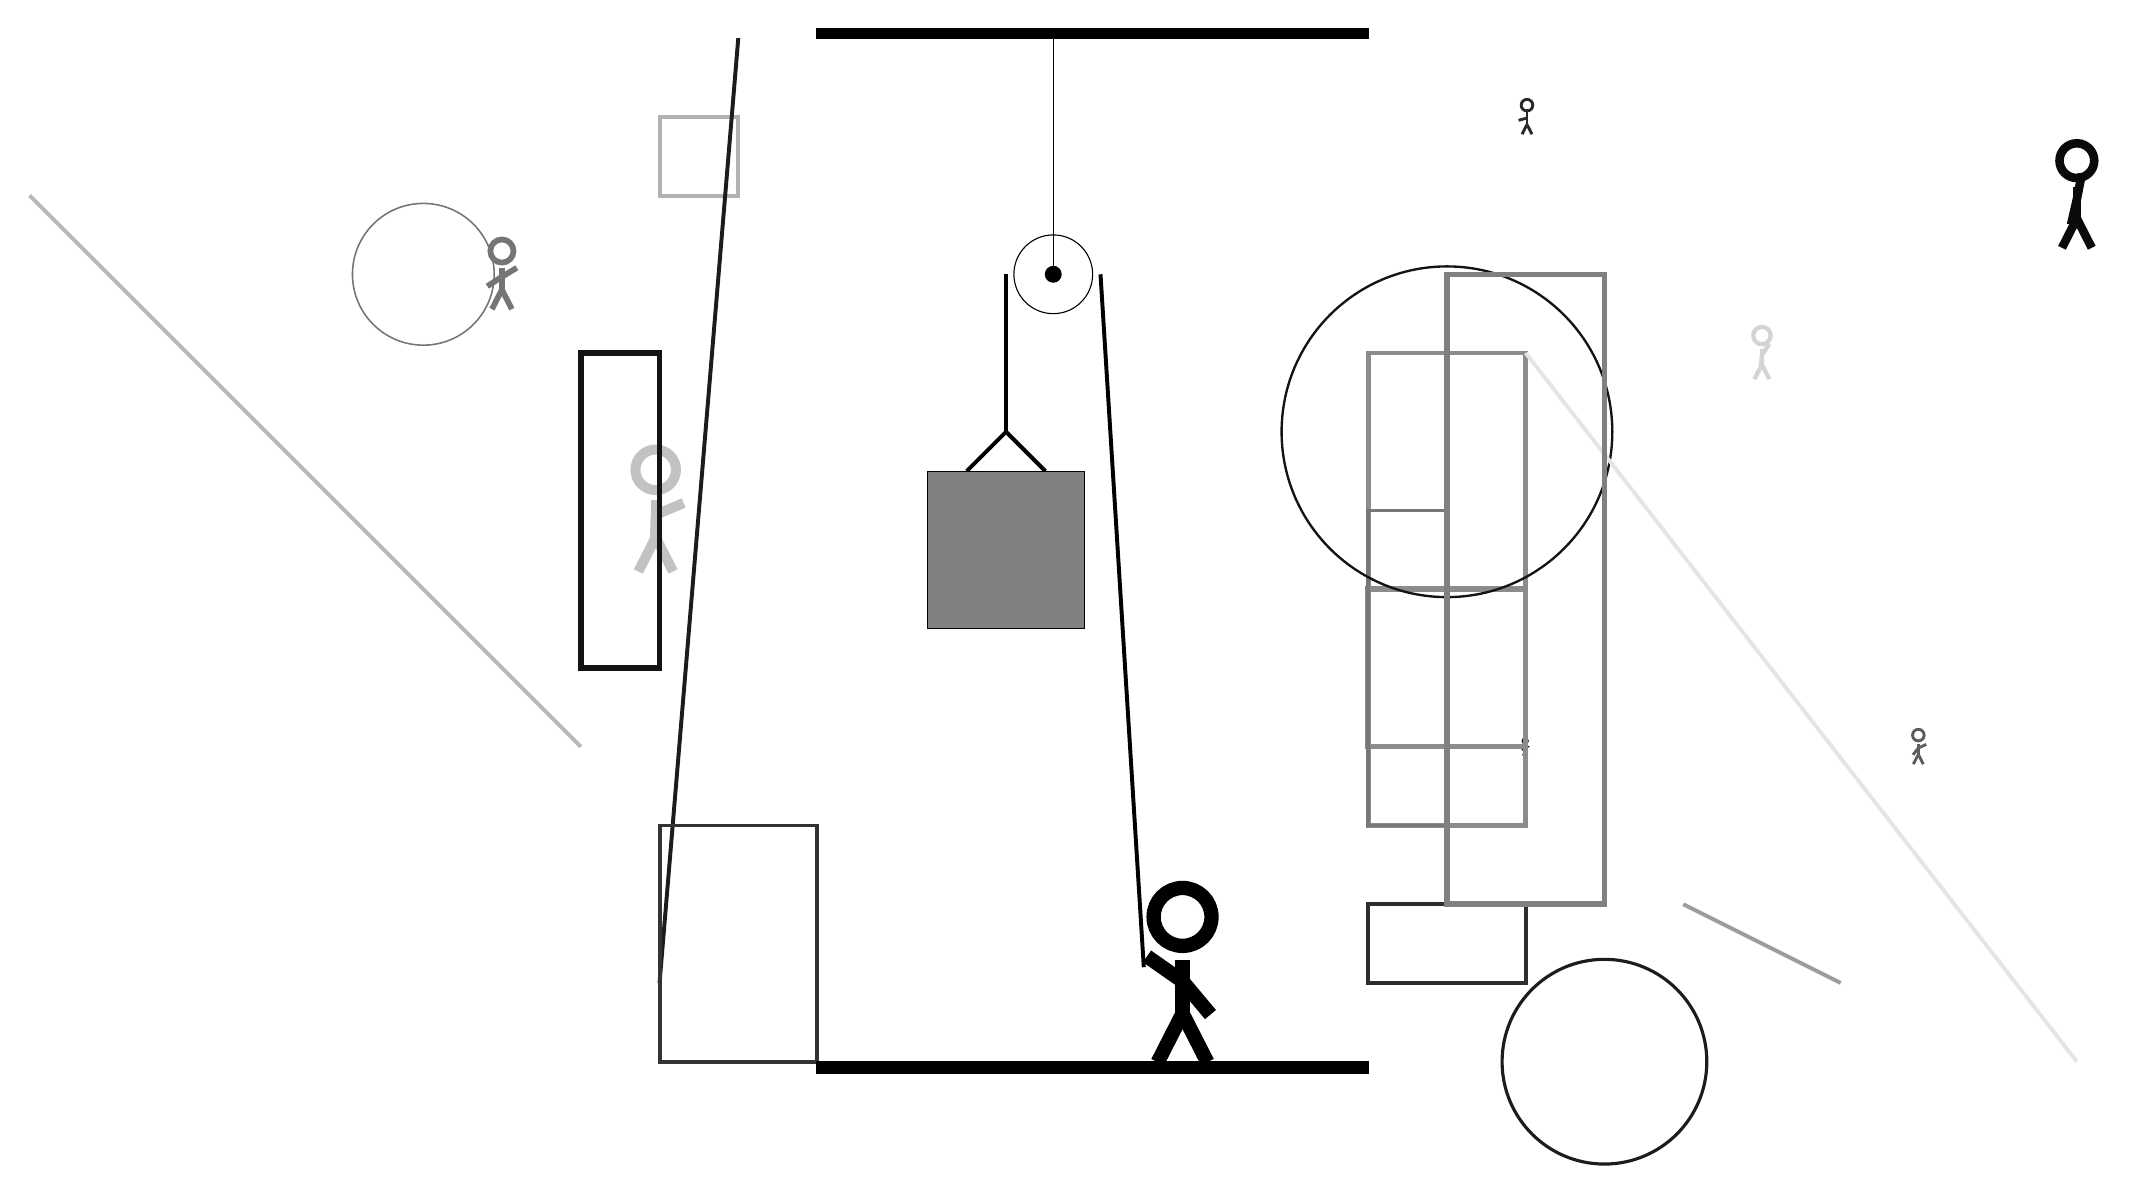
\begin{tikzpicture}
		%%%%% START %%%%%
		
		\draw[fill=black] (-2, 10) rectangle (5, 10.125);
		
		\draw (1, 7) circle (0.5);
		\draw[fill=black] (1, 7) circle (0.1);
		\draw (1, 10) -- (1, 7);
		
		\draw[line width=0.5mm] (-0.1, 4.5) -- (0.4, 5.0) -- (0.9, 4.5);
		\draw[fill=black!50] (-0.6, 4.5) rectangle (1.4, 2.5);
		
		\node[line width=0.3mm, color=black!91] at (7, 1) {\Strichmaxerl[1][42][11]};
		
		\draw [line width=0.4mm, color=black!89](8, -3) circle (1.3);
		\node[line width=0.3mm, color=black!17] at (10, 6) {\Strichmaxerl[3][85][56]};
		\draw[line width=0.5mm, color=black!39](9, -1) -- (11, -2);
		
		\draw [line width=0.2mm, color=black!54](-7, 7) circle (0.9);
		
		\draw[line width=0.5mm, color=black!82] (7, -2) rectangle (5, -1);
		
		\draw[line width=0.6mm, color=black!45] (7, 6) rectangle (5, 0);
		\node[line width=0.2mm, color=black!64] at (12, 1) {\Strichmaxerl[2][52][24]};
		\draw[line width=0.7mm, color=black!45] (7, 1) rectangle (5, 3);
		\draw[line width=0.5mm, color=black!30] (-3, 8) rectangle (-4, 9);
		\draw[line width=0.5mm, color=black!53] (6, 0) rectangle (5, 4);
		\draw[line width=0.5mm, color=black!28](-5, 1) -- (-12, 8);
		\node[line width=0.3mm, color=black!96] at (14, 8) {\Strichmaxerl[6][77][79]};
		
		\draw[line width=0.5mm, color=black!89](-3, 10) -- (-4, -2);
		\node[line width=0.7mm, color=black!84] at (7, 9) {\Strichmaxerl[2][15][90]};
		\node[line width=0.4mm, color=black!24] at (-4, 4) {\Strichmaxerl[7][88][23]};
		
		\draw [line width=0.3mm, color=black!92](6, 5) circle (2.1);
		\draw[line width=0.5mm, color=black!10](7, 6) -- (14, -3);
		\node[line width=0.3mm, color=black!54] at (-6, 7) {\Strichmaxerl[4][33][31]};
		
		\draw[line width=0.7mm, color=black!92] (-4, 6) rectangle (-5, 2);
		\draw[line width=0.7mm, color=black!50] (6, -1) rectangle (8, 7);
		
		\draw[line width=0.5mm, color=black!80] (-2, -3) rectangle (-4, 0);
		
		\draw[line width=0.5mm] (0.4, 7) -- (0.4, 5.0);
		\centerarc[line width=0.5mm](1, 7)(0:180:0.6);
		\draw[line width=0.5mm](1.6, 7) -- (2.15, -1.8);
		
		\node at (2.6, -1.9) {\Strichmaxerl[10][-35][-50]};
		
		\draw[fill=black] (-2, -3) rectangle (5, -3.15);
		
		%%%%% END %%%%%
	\end{tikzpicture}
\end{document}